
%\documentclass[justified, marginals=raggedouter]{tufte-handout}
\documentclass[justified, marginals=justified]{tufte-handout}

% Adding a few custom packages
\usepackage{tcolorbox}
\usepackage{lipsum}
\usepackage{bm,upgreek}
\usepackage{subfig}
% Example environment
\usepackage{amsthm}
\theoremstyle{definition}
\newtheorem{exmp}{Example}

% The default minimumo amount of space between \marginnotes is 10 pt.
\setlength\marginparpush{1cm}

\title{6.864 Advanced Natural Language Processing\thanks{Instructors: Prof. Regina Barzilay, and Prof. Tommi Jaakkola.\\ TAs: Franck Dernoncourt, Karthik Rajagopal Narasimhan, Tianheng Wang. \\ Scribes: Dongyoung Kim.}}

\author[Lecture 4: EM Algorithm and Topic Model]{Lecture 4: EM Algorithm and Topic Model}

\date{24 September 2015} % without \date command, current date is supplied

%\geometry{showframe} % display margins for debugging page layout

\usepackage{graphicx} % allow embedded images
  \setkeys{Gin}{width=\linewidth,totalheight=\textheight,keepaspectratio}
  \graphicspath{{graphics/}} % set of paths to search for images
\usepackage{amsmath}  % extended mathematics
\usepackage{booktabs} % book-quality tables
\usepackage{units}    % non-stacked fractions and better unit spacing
\usepackage{multicol} % multiple column layout facilities
\usepackage{lipsum}   % filler text
\usepackage{fancyvrb} % extended verbatim environments
  \fvset{fontsize=\normalsize}% default font size for fancy-verbatim environments

% Standardize command font styles and environments
\newcommand{\doccmd}[1]{\texttt{\textbackslash#1}}% command name -- adds backslash automatically
\newcommand{\docopt}[1]{\ensuremath{\langle}\textrm{\textit{#1}}\ensuremath{\rangle}}% optional command argument
\newcommand{\docarg}[1]{\textrm{\textit{#1}}}% (required) command argument
\newcommand{\docenv}[1]{\textsf{#1}}% environment name
\newcommand{\docpkg}[1]{\texttt{#1}}% package name
\newcommand{\doccls}[1]{\texttt{#1}}% document class name
\newcommand{\docclsopt}[1]{\texttt{#1}}% document class option name
\newenvironment{docspec}{\begin{quote}\noindent}{\end{quote}}% command specification environment

\begin{document}

\maketitle% this prints the handout title, author, and date

Earlier, we saw cases where the full data was observable and we could apply a straightforward maximum-likelihood estimator for the parameters. In Lecture 4, we introduce a Hidden Variable Model where data is partially observable. Then, we provide basic intuitions for the EM algorithm which can be used to optimize the likelihood on such Hidden Variable Models instead of directly solving it analytically. We explore further by demonstrating the EM algorithm on a toy example with biased coins. Later, we connect our concept to more relevant topics in NLP such as topic modeling.  

\section{Hidden Variable Models}\label{sec:hidden-variable-models}

\subsection{Motivation}\label{sec:motivation}

To gain intuition about Hidden Variable Models, see the following examples. 

\begin{enumerate}
	\item \textit{Topic model}: Consider the following unigram model; A topic is denoted by $z$ where $z\in\mathcal{Z}$, and $\mathcal{Z}$ is our pre-defined universe of topics of $k$ dimension. The document $D$ is comprised of $N$ words such that $D=\{w_1, w_2, ..., w_N\}$. Each word $w_i$ is sampled from a corresponding topic $z_i$. If the entire data had been observed, we could simply estimate the conditional distribution as the empirical count,
	\begin{align}
	\hat{p}(w|z) = \dfrac{count(w,z)}{count(z)}
	\end{align}
	
		\begin{marginfigure}[-3cm]%
			\centering
			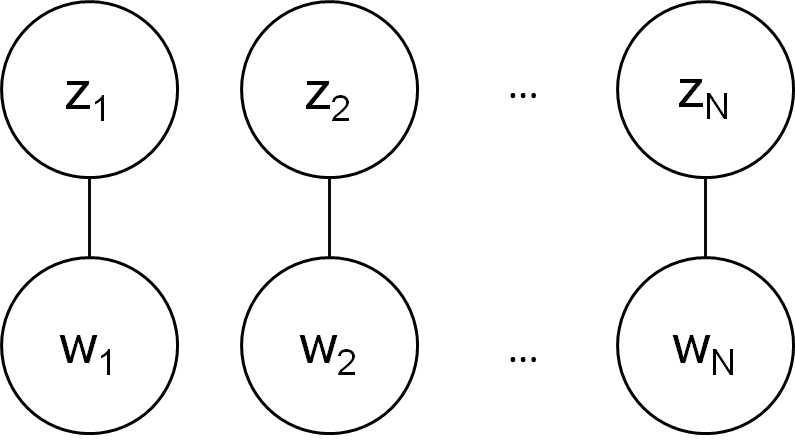
\includegraphics[width=4cm]{topic-model-unigram.png}
			\caption{Topic model is where each word is associated with a conditional topic. For example, it is more likely to observe word $w_i="Cat"$ if the topic is $z_i="Pets"$.}
			\label{fig:topic-model-unigram}
		\end{marginfigure}
	
	However, such straightforward approach seen in (1) is no longer applicable if the variables $z_i$ are hidden. Since it is unlikely to have each word in a document explicitly tagged with its related topics, topic models naturally arise as Hidden Variable Models.
	
	\item \textit{Machine Translation Alignment}: 
	In Machine Translation, one is given two sentences in different languages with the same meaning. As seen in Figure~\ref{fig:machine-translation-alignment}, when the word \textit{"I"} is paired together many times with the corresponding Korean word, then it is probably a good indicator that \textit{"I"} should be translated to that word. Therefore, the first step in Machine Translation is to align corresponding translations. However, the alignments are not explicitly given in real life applications and should be treated as hidden variables one has to estimate. 
		\begin{marginfigure}[-3cm]%
			\centering
			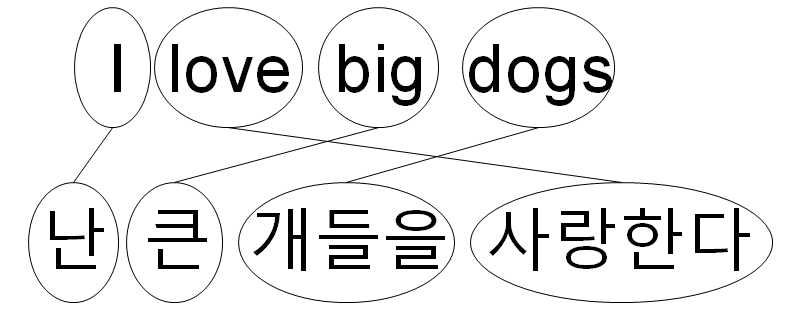
\includegraphics[width=4cm]{machine-translation-alignment.png}
			\caption{In machine translation, each word from one language has a hidden alignment to its counterpart.}
			\label{fig:machine-translation-alignment}
		\end{marginfigure}	

	\item \textit{Part-of-Speech Tagging}: Part-of-speech tagging, which will be covered in the next lecture, matches each word in a sentence with its part of speech in English. For the example in Figure~\ref{fig:machine-translation-alignment}, \textit{"I"} is tagged with \textit{"pronoun"}, \textit{"love"} with \textit{"verb"}, \textit{"big"} with \textit{"adjective"}, and \textit{"dogs"} with \textit{"noun"}. When the full observed data observable, one can apply a supervised learning algorithm. However when the parts of speech are not observed, then they are treated as hidden variables. 
\end{enumerate}

\subsection{Observed Case vs. Unobserved Case}\label{sec:observed-case-vs-unobserved-case}

In previous lectures we looked at models where the full data was observed. We use 
\begin{align*}
D = \{(x_1, y_1), (x_2, y_2), ..., (x_N, y_N)\}
\end{align*}

\noindent to denote the given dataset in such cases, which is represented as a list of sampled tuples. Each data point $(x, y)$ is independently sampled from some distribution $p_{\text{X,Y}}(x,y)$ parameterized by $\theta$. The objective function we are trying to maximize is given by the following
\begin{align}
\label{eq:observed}\theta^{*} = \underset{\theta}{\operatorname{argmax}}\sum_{i=1}^{N}\log{p_{\text{X,Y}}(x_i, y_i|\theta) }
\end{align}

Now, let's look at the unobserved case where $\textbf{y}$ is unseen. In other words, $\textbf{x}$ is the observed variable and $\textbf{y}$ is the hidden variable. In this case, the observed data is given by
\begin{align*}
D = \{x_1, x_2, ..., x_N\}
\end{align*}
In this case, we replace the objective function with the log-likelihood of the \textit{partially observed data}, which is
\begin{align}
\theta^{*} &= \underset{\theta}{\operatorname{argmax}}\sum_{i=1}^{N}\log{p_{\text{X}}(x_i|\theta) } \nonumber \\
\label{eq:unobserved}&= \underset{\theta}{\operatorname{argmax}}\sum_{i=1}^{N}\log\sum_{y\in \mathcal{Y}}p_{\text{X,Y}}(x_i, y|\theta)
\end{align} 

\noindent where the second equality is due to marginalization over $y$ over $p_{ \text{X,Y} }(x,y)$. The key point is to note that the criteria for the observed case and the unobserved case is different, and we should use a different objective function when we are trying to optimize for the parameter $\theta$. In the following sections we will demonstrate how the EM algorithm finds the optimum parameter for (\ref{eq:unobserved}).

\section{EM Algorithm}\label{sec:em-algorithm}
\begin{exmp}\label{exmp1}

We will set up a simple example to walk through how the EM algorithm works. Suppose we have a card and two different coins, where all probabilities are biased. We will take the following steps to sample a sequence of coin flips.
\begin{enumerate}
	\item Flip the card, which either returns side \textit{A} or side \textit{B}.
	\item If \textit{A} was drawn from step 1, toss coin \text{1} three times. Otherwise if \textit{B} was drawn, toss coin 2 three times. 
	\item repeat steps 1-2
\end{enumerate}

Expressing this more formally, $y$ represents the side of the card and $x$ represents the outcome of three consecutive coin tosses. $H$ and $T$ denotes the head and tail of a coin, respectively. 
\begin{align*}
y \in \mathcal{Y} &= \{A, B\} \\*
x \in \mathcal{X} &= \{HHH, HTH, ..., TTT\}
\end{align*}
There are three free parameters in this setup, given by $\bm\uptheta = \{\alpha, \pi_1, \pi_2 \}$. The parameters are described as follows
\begin{align*}
\alpha &= p(Card = A) \\*
\pi_1 &= p(Coin 1 = H) \\*
\pi_2 &= p(Coin 2 = H) 
\end{align*}
It is easy to see that
\begin{align*}
p_{\text{X,Y}}(x,y|\bm\uptheta) &= p_{\text{Y}}(y|\bm\uptheta)p_{\text{X|Y}}(x|y,\bm\uptheta) \\*
p_{\text{Y}}(y|\bm\uptheta) &= \left\{ 
	\begin{array}{l l}
		\alpha & \quad \text{if $y = A$}\\
		1-\alpha & \quad \text{if $y = B	$}
	\end{array} \right.\\*
p_{\text{X|Y}}(x|y,\bm\uptheta) &= \left\{ 
	\begin{array}{l l}
		\pi_1^{h(x)}(1-\pi_1)^{t(x)} & \quad \text{if $y = A$}\\
		\pi_2^{h(x)}(1-\pi_2)^{t(x)} & \quad \text{if $y = B	$}
	\end{array} \right.
\end{align*}

Where we define $h(x)$ to be a function that is equal to the number of heads in sample $x$, and $t(x)$ to be the number of tails. For example, if $x_0 = {HHT}$, then $h(x_0) = 2$ and $t(x_0) = 1$.  

\end{exmp}

\subsection{Observed Case}\label{sec:observed-case}
In the observed case, the card flips and the coin tosses are entirely observable. Each card flip is associated with three coin tosses. Suppose after three iterations, the sampled data was given as follows
\begin{align*}
D = \{(A, HHH), (A, HHH), (B, TTT)\}
\end{align*}

where $(y,x) = (A, HHH)$ denotes that the observed card flip was $A$, followed by three heads. We had seen in earlier lectures that applying partial derivative to the log-likelihood given in \eqref{eq:observed}, the MLE parameters are simply given by the empirical counts. Using this fact for granted, the parameter values for these specific samples are given by
\begin{align*}
\alpha^{*} &= \dfrac{\text{count(A)}}{3}=\dfrac{2}{3} \\*
\pi_1^{*} &= \dfrac{ \text{count}(A,H)} { \text{count}(A, H)+\text{count}(A, T) } = \dfrac{6}{6} \\*
\pi_2^{*} &= \dfrac{ \text{count}(B,H)} { \text{count}(B, H)+\text{count}(B, T) } = \dfrac{0}{3}
\end{align*}
Shortly we will see that this analytic solution has a very similar form to the solution for each iteration in the EM algorithm, which is covered in the next section. 

\subsection{Unobserved Case}\label{sec:unobserved-case}

Continuing with the problem setup in Example \ref{exmp1}, suppose the card flips are no longer observable. In other words, we will treat the card flip $y$ as a hidden variable. Consider the following sample data
\begin{align*}
D = \{HHH, HHH, TTT\} = \textbf{x}
\end{align*}

Let us make an initial guess on the parameter values. Assign arbitrary prior values such that 
\begin{align}
\label{priors}
\alpha^{(0)} = 0.1,\quad \pi_1^{(0)}=0.8,\quad \pi_2^{(0)}=0.5\quad
\end{align}
The initial guess in (\ref{priors}) is denoted with a superscript 0 to mark that this is the belief of the parameters at time 0. We will see how the belief is updated over each iteration of the EM algorithm. 

For each $x_i $ in the dataset, we compute $p_{\text{Y|X}, \bm\uptheta}(y|x_i, \bm{\uptheta}^{(0)})$ over all possible values of $y \in \mathcal{Y} = \{A, B\}$.  For example, for our  For $x_1 = HHH$ in the given example dataset,
\vspace{3mm} \\
\begin{math}
\-\hspace{0ex} p_{\text{Y|X}, \bm\uptheta}(y_1=A|x_1=HHH, \bm{\uptheta}^{(0)}) \\
\-\hspace{0ex} = \dfrac { p_{\text{X, Y}| \bm\uptheta}(x_1=HHH, y_1=A | \bm{\uptheta}^{(0)}) }
{p_{\text{X, Y}| \bm\uptheta}(x_1=HHH, y_1=A | \bm{\uptheta}^{(0)})+p_{\text{X, Y}| \bm\uptheta}(x_1=HHH, y_1=B | \bm{\uptheta}^{(0)})} \\*
\-\hspace{0ex} = \dfrac{ \alpha\pi_1^3 }{ \alpha\pi_1^3 + (1-\alpha)\pi_2^3 } \vspace{2mm} \\*
\-\hspace{0ex} \approx 0.3  \\*
\-\hspace{0ex} p_{\text{Y|X}, \bm\uptheta}(y_1=B|x_1=HHH, \bm{\uptheta}^{(0)}) \\  %equation2
\-\hspace{0ex} = \dfrac{ p_{\text{X, Y}| \bm\uptheta}(x_1=HHH, y_1=B | \bm{\uptheta}^{(0)}) }
{p_{\text{X, Y}| \bm\uptheta}(x_1=HHH, y_1=A | \bm{\uptheta}^{(0)})+p_{\text{X, Y}| \bm\uptheta}(x_1=HHH, y_1=B | \bm{\uptheta}^{(0)})} \\*
\-\hspace{0ex} = \dfrac{ (1-\alpha)\pi_2^3 }{ \alpha\pi_1^3 + (1-\alpha)\pi_2^3 } \vspace{2mm} \\*
\-\hspace{0ex} \approx 0.7
\end{math}
\vspace{3mm} \\
Recall from the previous section that in the fully observed case, each $x_i$ was explicitly associated with a \textit{single} count of either $y_i=A$ or $y_i=B$. In the unobserved case, we assume that each $x_i$ is associated with \textit{fractional counts} over all possible values of $y_i$, to which we assign the \textit{expected count} of $y_i$ given $x_i$ and our prior knowledge of $\bm{\uptheta}$, i.e. $\mathbb{E}[y|x=x_i, \bm{\uptheta}^{(0)}]$.

\begin{table}[h]
	\centering
	\subfloat[$y$ is observed]{
		\begin{tabular}{ccc}
			\toprule
			$x_i$ & $y_i$ & empirical count \\
			\midrule
			HHH & A & 1 \\
			 &  &  \\
			HHH & A & 1 \\
			 &  &  \\
			TTT & B & 1 \\
			 &  &  \\
			\bottomrule
		\end{tabular}
	}
	\quad
	\subfloat[$y$ is unobserved]{
		\begin{tabular}{ccc}
			\toprule
			$x_i$ & $y_i$ & fractional count \\
			\midrule
			HHH & A & 0.3 \\
			  & B & 0.7 \\
			HHH & A & 0.3 \\
			& B & 0.7 \\
			TTT & A & 0.5 \\
			& B & 0.5 \\
			\bottomrule
		\end{tabular}
	}
	\caption{In the fully observed case (a), a single value of $y$ (which is the observed value itself) is associated with each $i^{\text{th}}$ data sample. In the unobserved case (b), we assume that a entire list over the alphabet $\mathcal{Y}$, is associated with $x_i$. Each element in the spectrum is assigned a weight, or the \textit{fractional count}, which corresponds to the expected value of $y$ given $x_i$. The fractional count can also be understood as the confidence in the sample ($x_i, y_i$) given a prior belief over the parameters. }
\end{table}

\vspace{3ex}
Hereafter the remaining steps are almost identical to the MLE maximization of the parameters. Again we will derive our distribution by counting, but since the actual counts are no longer given, we will count the fractional counts instead. The parameters for the next iteration, or time 1, will be computed as follows
\begin{align*}
\alpha^{(1)}&\leftarrow \dfrac{\text{fractional count of }A}{3} = \dfrac{0.3+0.3+0.5}{3}= \dfrac{1.1}{3} \\*
\pi_1^{(1)}&\leftarrow \dfrac{\text{fractional count of }(A, H)}{\text{fractional count of }(A, H) + \text{fractional count of }(A, T)} \\*
& = \dfrac{3\times0.3 + 3\times0.3}{3\times0.3 + 3\times0.3+3\times0.5}= \dfrac{1.8}{3.3} \\*
\pi_2^{(1)}&\leftarrow \dfrac{\text{fractional count of }(B, H)}{\text{fractional count of }(B, H) + \text{fractional count of }(B, T)} \\*
& = \dfrac{ 3\times0.7 + 3\times0.7 }{ 3\times0.7 + 3\times0.7 + 3\times0.5}= \dfrac{4.2}{5.7}
\end{align*}

The EM algorithm guarantees that the likelihood given by Equation (\ref{eq:unobserved}) is increased over every iteration as we update our parameters $\bm{\uptheta}^{(0)}, \bm{\uptheta}^{(1)}, 
\bm{\uptheta}^{(2)}, ..., \bm{\uptheta}^{(T)}$. In summary, the EM algorithm is given by the following steps

\begin{enumerate}
	\item
	Randomly initialize $\bm{\uptheta}^{(0)}$
	\item
	Based on $\bm{\uptheta}^{(t)}$, compute $p_(y|x, \bm{\uptheta}^{(t)})$ and count the fractionals
	\item
	Re-estimate $\bm{\uptheta}^{(t+1)}$
	\item
	Repeat until convergence
\end{enumerate}

\subsection{Properties of EM Algorithms}

We can make the following soft statements about the EM algorithm's behavior

\begin{enumerate}
	\item
	 The algorithm converges to a stationary point
	\item
	The algorithm converges to a local maximum
\end{enumerate}

On final note, when $y$ is hidden, it is also likely that we do not have previous knowledge of the alphabet space $\mathcal{Y}$. The selection of the alphabet space is treated as a regularization problem, similar to selecting the number of units in a neural network, which will be optimized by cross-validation over a development data set. 

\section{Topic Model}\label{sec:topic-model}

\begin{table}[h]
	\centering
	\caption{For each given topic, some words are more likely to appear than others}
	\begin{tabular}{cccc}
		\toprule
		"Art" & "Budget" & "Children" & "Education"  \\
		\midrule
		new & money & care & state \\
		film & congress & percent & president \\
		show & & family & schools \\
		& & welfare & Haiti \\
		\bottomrule \\
	\end{tabular}
\end{table}

\subsection{Introduction to Topic Model} 
In this section, we will briefly introduce Topic Model. Consider a simple unigram model where the probability of a word $w_i$ is given by $p(w_i)=\theta_i$. We will also model a topic $z$ such that $z\in\mathcal{Z}$ and $|\mathcal{Z}=k|$, where $\mathcal{Z}$ is our universe of topics and the dimension $k$ is treated as a hyperparameter. Each word in the document will be generated from the distribution $p(w_i|z) = \theta_{w_i|z}$, according to the following steps
\begin{enumerate}
	\item Sample a topic $z$
	\item Generate the entire document with the given topic
\end{enumerate}

Then, the likelihood of the document $d$ of size $N$ can be expressed as
\begin{align*}
p(d|\bm{\uptheta}) = \sum_{z\in\mathcal{Z}}\theta_z\prod_{i=1}^{N}\theta_{w_i|z}
\end{align*}
However, this model is problematic because it assumes that the whole document comes from a single topic. In real-life, it is more likely that topics may change throughout the document. Motivated by this approach, we setup a new model where each word $w_i$ is sampled from each corresponding topic $z_i$. The sampling procedure will now be
\begin{enumerate}
	\item Sample a topic $z_i$
	\item Sample a word $w_i$ conditional on $z_i$
	\item Sample the next topic $z_{i+1}$
	\item Repeat until end of document.
\end{enumerate}

The likelihood for the new model is
\begin{align*}
p_(d|\bm{\uptheta})=\prod_{i=1}^{N}\sum_{z\in\mathcal{Z}}\theta_{z|d}\theta_{w_i|z}
\end{align*}

The distribution over the topics is unique for each document, represented by $\theta_{z|d}$. Across all documents, the word conditional on a given topic is sampled from a single "shared" distribution, represented by $\theta_{w|z}$. It is easy to see that if both the words and topics are fully observed, we can derive the MLE parameters by looking at the empirical distributions
\begin{align*}
\hat{\theta}_{w_i|z} &= \dfrac{\text{count}(w_i,z)}{\text{count}(z)} \\*
\hat{\theta}_{z|d} &= \dfrac{\text{count}(z)}{N}
\end{align*}

In application, however, topic information are not given out in the training data and the problem should be treated as a Hidden Variable Model. We leave it to the readers to think about how the EM algorithm can be applied to solve this specific unigram topic model. 

\end{document}
